% Options for packages loaded elsewhere
\PassOptionsToPackage{unicode}{hyperref}
\PassOptionsToPackage{hyphens}{url}
\PassOptionsToPackage{dvipsnames,svgnames,x11names}{xcolor}
%
\documentclass[
  letterpaper,
  DIV=11,
  numbers=noendperiod]{scrartcl}

\usepackage{amsmath,amssymb}
\usepackage{iftex}
\ifPDFTeX
  \usepackage[T1]{fontenc}
  \usepackage[utf8]{inputenc}
  \usepackage{textcomp} % provide euro and other symbols
\else % if luatex or xetex
  \usepackage{unicode-math}
  \defaultfontfeatures{Scale=MatchLowercase}
  \defaultfontfeatures[\rmfamily]{Ligatures=TeX,Scale=1}
\fi
\usepackage{lmodern}
\ifPDFTeX\else  
    % xetex/luatex font selection
\fi
% Use upquote if available, for straight quotes in verbatim environments
\IfFileExists{upquote.sty}{\usepackage{upquote}}{}
\IfFileExists{microtype.sty}{% use microtype if available
  \usepackage[]{microtype}
  \UseMicrotypeSet[protrusion]{basicmath} % disable protrusion for tt fonts
}{}
\makeatletter
\@ifundefined{KOMAClassName}{% if non-KOMA class
  \IfFileExists{parskip.sty}{%
    \usepackage{parskip}
  }{% else
    \setlength{\parindent}{0pt}
    \setlength{\parskip}{6pt plus 2pt minus 1pt}}
}{% if KOMA class
  \KOMAoptions{parskip=half}}
\makeatother
\usepackage{xcolor}
\setlength{\emergencystretch}{3em} % prevent overfull lines
\setcounter{secnumdepth}{5}
% Make \paragraph and \subparagraph free-standing
\makeatletter
\ifx\paragraph\undefined\else
  \let\oldparagraph\paragraph
  \renewcommand{\paragraph}{
    \@ifstar
      \xxxParagraphStar
      \xxxParagraphNoStar
  }
  \newcommand{\xxxParagraphStar}[1]{\oldparagraph*{#1}\mbox{}}
  \newcommand{\xxxParagraphNoStar}[1]{\oldparagraph{#1}\mbox{}}
\fi
\ifx\subparagraph\undefined\else
  \let\oldsubparagraph\subparagraph
  \renewcommand{\subparagraph}{
    \@ifstar
      \xxxSubParagraphStar
      \xxxSubParagraphNoStar
  }
  \newcommand{\xxxSubParagraphStar}[1]{\oldsubparagraph*{#1}\mbox{}}
  \newcommand{\xxxSubParagraphNoStar}[1]{\oldsubparagraph{#1}\mbox{}}
\fi
\makeatother

\usepackage{color}
\usepackage{fancyvrb}
\newcommand{\VerbBar}{|}
\newcommand{\VERB}{\Verb[commandchars=\\\{\}]}
\DefineVerbatimEnvironment{Highlighting}{Verbatim}{commandchars=\\\{\}}
% Add ',fontsize=\small' for more characters per line
\usepackage{framed}
\definecolor{shadecolor}{RGB}{241,243,245}
\newenvironment{Shaded}{\begin{snugshade}}{\end{snugshade}}
\newcommand{\AlertTok}[1]{\textcolor[rgb]{0.68,0.00,0.00}{#1}}
\newcommand{\AnnotationTok}[1]{\textcolor[rgb]{0.37,0.37,0.37}{#1}}
\newcommand{\AttributeTok}[1]{\textcolor[rgb]{0.40,0.45,0.13}{#1}}
\newcommand{\BaseNTok}[1]{\textcolor[rgb]{0.68,0.00,0.00}{#1}}
\newcommand{\BuiltInTok}[1]{\textcolor[rgb]{0.00,0.23,0.31}{#1}}
\newcommand{\CharTok}[1]{\textcolor[rgb]{0.13,0.47,0.30}{#1}}
\newcommand{\CommentTok}[1]{\textcolor[rgb]{0.37,0.37,0.37}{#1}}
\newcommand{\CommentVarTok}[1]{\textcolor[rgb]{0.37,0.37,0.37}{\textit{#1}}}
\newcommand{\ConstantTok}[1]{\textcolor[rgb]{0.56,0.35,0.01}{#1}}
\newcommand{\ControlFlowTok}[1]{\textcolor[rgb]{0.00,0.23,0.31}{\textbf{#1}}}
\newcommand{\DataTypeTok}[1]{\textcolor[rgb]{0.68,0.00,0.00}{#1}}
\newcommand{\DecValTok}[1]{\textcolor[rgb]{0.68,0.00,0.00}{#1}}
\newcommand{\DocumentationTok}[1]{\textcolor[rgb]{0.37,0.37,0.37}{\textit{#1}}}
\newcommand{\ErrorTok}[1]{\textcolor[rgb]{0.68,0.00,0.00}{#1}}
\newcommand{\ExtensionTok}[1]{\textcolor[rgb]{0.00,0.23,0.31}{#1}}
\newcommand{\FloatTok}[1]{\textcolor[rgb]{0.68,0.00,0.00}{#1}}
\newcommand{\FunctionTok}[1]{\textcolor[rgb]{0.28,0.35,0.67}{#1}}
\newcommand{\ImportTok}[1]{\textcolor[rgb]{0.00,0.46,0.62}{#1}}
\newcommand{\InformationTok}[1]{\textcolor[rgb]{0.37,0.37,0.37}{#1}}
\newcommand{\KeywordTok}[1]{\textcolor[rgb]{0.00,0.23,0.31}{\textbf{#1}}}
\newcommand{\NormalTok}[1]{\textcolor[rgb]{0.00,0.23,0.31}{#1}}
\newcommand{\OperatorTok}[1]{\textcolor[rgb]{0.37,0.37,0.37}{#1}}
\newcommand{\OtherTok}[1]{\textcolor[rgb]{0.00,0.23,0.31}{#1}}
\newcommand{\PreprocessorTok}[1]{\textcolor[rgb]{0.68,0.00,0.00}{#1}}
\newcommand{\RegionMarkerTok}[1]{\textcolor[rgb]{0.00,0.23,0.31}{#1}}
\newcommand{\SpecialCharTok}[1]{\textcolor[rgb]{0.37,0.37,0.37}{#1}}
\newcommand{\SpecialStringTok}[1]{\textcolor[rgb]{0.13,0.47,0.30}{#1}}
\newcommand{\StringTok}[1]{\textcolor[rgb]{0.13,0.47,0.30}{#1}}
\newcommand{\VariableTok}[1]{\textcolor[rgb]{0.07,0.07,0.07}{#1}}
\newcommand{\VerbatimStringTok}[1]{\textcolor[rgb]{0.13,0.47,0.30}{#1}}
\newcommand{\WarningTok}[1]{\textcolor[rgb]{0.37,0.37,0.37}{\textit{#1}}}

\providecommand{\tightlist}{%
  \setlength{\itemsep}{0pt}\setlength{\parskip}{0pt}}\usepackage{longtable,booktabs,array}
\usepackage{calc} % for calculating minipage widths
% Correct order of tables after \paragraph or \subparagraph
\usepackage{etoolbox}
\makeatletter
\patchcmd\longtable{\par}{\if@noskipsec\mbox{}\fi\par}{}{}
\makeatother
% Allow footnotes in longtable head/foot
\IfFileExists{footnotehyper.sty}{\usepackage{footnotehyper}}{\usepackage{footnote}}
\makesavenoteenv{longtable}
\usepackage{graphicx}
\makeatletter
\def\maxwidth{\ifdim\Gin@nat@width>\linewidth\linewidth\else\Gin@nat@width\fi}
\def\maxheight{\ifdim\Gin@nat@height>\textheight\textheight\else\Gin@nat@height\fi}
\makeatother
% Scale images if necessary, so that they will not overflow the page
% margins by default, and it is still possible to overwrite the defaults
% using explicit options in \includegraphics[width, height, ...]{}
\setkeys{Gin}{width=\maxwidth,height=\maxheight,keepaspectratio}
% Set default figure placement to htbp
\makeatletter
\def\fps@figure{htbp}
\makeatother

\KOMAoption{captions}{tableheading}
\makeatletter
\@ifpackageloaded{caption}{}{\usepackage{caption}}
\AtBeginDocument{%
\ifdefined\contentsname
  \renewcommand*\contentsname{Table of contents}
\else
  \newcommand\contentsname{Table of contents}
\fi
\ifdefined\listfigurename
  \renewcommand*\listfigurename{List of Figures}
\else
  \newcommand\listfigurename{List of Figures}
\fi
\ifdefined\listtablename
  \renewcommand*\listtablename{List of Tables}
\else
  \newcommand\listtablename{List of Tables}
\fi
\ifdefined\figurename
  \renewcommand*\figurename{Figure}
\else
  \newcommand\figurename{Figure}
\fi
\ifdefined\tablename
  \renewcommand*\tablename{Table}
\else
  \newcommand\tablename{Table}
\fi
}
\@ifpackageloaded{float}{}{\usepackage{float}}
\floatstyle{ruled}
\@ifundefined{c@chapter}{\newfloat{codelisting}{h}{lop}}{\newfloat{codelisting}{h}{lop}[chapter]}
\floatname{codelisting}{Listing}
\newcommand*\listoflistings{\listof{codelisting}{List of Listings}}
\makeatother
\makeatletter
\makeatother
\makeatletter
\@ifpackageloaded{caption}{}{\usepackage{caption}}
\@ifpackageloaded{subcaption}{}{\usepackage{subcaption}}
\makeatother

\ifLuaTeX
  \usepackage{selnolig}  % disable illegal ligatures
\fi
\usepackage{bookmark}

\IfFileExists{xurl.sty}{\usepackage{xurl}}{} % add URL line breaks if available
\urlstyle{same} % disable monospaced font for URLs
\hypersetup{
  pdftitle={McKinney Fire metabolism: Model comparisons and QA},
  pdfauthor={Laurel Genzoli},
  colorlinks=true,
  linkcolor={blue},
  filecolor={Maroon},
  citecolor={Blue},
  urlcolor={Blue},
  pdfcreator={LaTeX via pandoc}}


\title{McKinney Fire metabolism: Model comparisons and QA}
\author{Laurel Genzoli}
\date{2025-07-29}

\begin{document}
\maketitle

\renewcommand*\contentsname{Table of contents}
{
\hypersetup{linkcolor=}
\setcounter{tocdepth}{3}
\tableofcontents
}

\section{Script Description}\label{script-description}

This script contains the streamMetabolizer model diagnostics for year
round data at Seiad Valley from 2018-2023. This is the minimal
reproducible code that shows how we assessed the output of the
metabolism model and what data we flagged to exclude from our analysis.

We first ran the model using the Bayesian solution in sM, and assessed
the output from this model. We found variation in K600 that was still
more than we would like (due to issues with how sM essentially ignores
priors and brings in more day to day variation than what is likely based
on discharge variation). After assessing the model output and finding it
to be overall good (with the exception of K600 variation being less than
ideal), we used the K600 output to ``hand pool'' K600 using a Loess
relationship between K600 and discharge. Then we assigned a K600 value
to each day based on Q, and reran the model using the MLE solution with
a fixed value for K600.

In our model assessments, we looked at the following and flagged data to
exclude from our analysis when the model did not perform well on a given
day. While we considered model convergence and model fits in the Bayes
run before using the K600 values to hand-pool K600 in our MLE run, we
found the data set to be very good overall, and the few outlier points
in K600 have very little effect on the relationship between K600 and
flow, so we retained all K600 estimates at this step.

In our MLE run (final estimates), we compared the outcomes to the Bayes
run, looked at model fits along side realistic values of ER and GPP, and
we examined days were GPP and ER were negative and positive
respectively. We excluded ER when daily DO was supersaturated for the
full day because this causes ER to be estimated as positive. We then
applied QA codes to MLE data set to exclude these days from the
analysis. We scaled the metabolism data to depth, and added covariates
to this data frame for further analysis presented within the final
manuscript.

\section{Load packages and data}\label{load-packages-and-data}

\subsection{Packages}\label{packages}

\begin{Shaded}
\begin{Highlighting}[]
\FunctionTok{setwd}\NormalTok{(}\StringTok{\textquotesingle{}/Users/laurelgenzoli/Dropbox/2024\_Projects/Mckinney\_Fire\_Metab/Mck{-}Fire{-}Metab{-}GH\textquotesingle{}}\NormalTok{)}

\FunctionTok{library}\NormalTok{(tidyverse)}
\FunctionTok{library}\NormalTok{(lubridate)}
\FunctionTok{library}\NormalTok{(dataRetrieval)}
\FunctionTok{library}\NormalTok{(viridis)}
\FunctionTok{library}\NormalTok{(cowplot)}
\FunctionTok{library}\NormalTok{(ggpubr)}
\FunctionTok{library}\NormalTok{(streamMetabolizer)}
\FunctionTok{library}\NormalTok{(hms)}
\FunctionTok{library}\NormalTok{(plotly)}
\FunctionTok{library}\NormalTok{(timeDate)}
\FunctionTok{library}\NormalTok{(zoo)}

\FunctionTok{theme\_set}\NormalTok{(}\FunctionTok{theme\_classic}\NormalTok{())}
\end{Highlighting}
\end{Shaded}

\subsection{Data}\label{data}

\subsubsection{Flow data}\label{flow-data}

\begin{itemize}
\tightlist
\item
  Discharge at SV and IG
\item
  Downloaded using dataRetrieval
\end{itemize}

\small

\normalsize

\subsubsection{Sonde data}\label{sonde-data}

\begin{itemize}
\tightlist
\item
  Water quality data (the cleaned sonde file that was used in metab
  calcs)
\item
  Does not have Turbidity data included in this df
\item
  This data is held by the Karuk Tribe and request for this raw water
  quality data needs to be made directly to the Karuk DNR
\end{itemize}

\small

\normalsize

\subsubsection{Sonde data with all parameters for daily
stats:}\label{sonde-data-with-all-parameters-for-daily-stats}

\begin{itemize}
\tightlist
\item
  The other water quality parameters (sc, Turb, pH) have not been QA'd
  visually
\item
  We didn't end up analyzing other water quality in this project; just
  turb and DO
\item
  Data was started late Oct 2018; update with turb data from May 2018
\item
  No need for other WQ data in this analysis; just sub for full time
  period turbidity data
\item
  Missing turb data is minimal and wont change analysis-not going to
  interpolate
\item
  similar to Sonde file above, this data is held by the Karuk Tribe and
  request for this raw water quality data needs to be made directly to
  the Karuk DNR
\item
  The final file here is ``sv.wq'' and has daily stats for wq parameters
\end{itemize}

\small

\begin{verbatim}
 [1] "date"              "turb_min"          "turb_mean"        
 [4] "turb_median"       "turb_max"          "turb_range"       
 [7] "temp.water_min"    "temp.water_mean"   "temp.water_median"
[10] "temp.water_max"    "temp.water_range"  "sc_min"           
[13] "sc_mean"           "sc_median"         "sc_max"           
[16] "sc_range"          "domg_min"          "domg_mean"        
[19] "domg_median"       "domg_max"          "domg_range"       
[22] "ph_min"            "ph_mean"           "ph_median"        
[25] "ph_max"            "ph_range"         
\end{verbatim}

\normalsize

\subsubsection{Metabolism data from Bayes
run}\label{metabolism-data-from-bayes-run}

\begin{itemize}
\tightlist
\item
  Metabolism output
\item
  Model fit and diagnostics files
\end{itemize}

\small

\normalsize

\subsubsection{Metabolism data from MLE run with ``hand-pooled''
K600}\label{metabolism-data-from-mle-run-with-hand-pooled-k600}

Similar to above but for the MLE run which used the gas exchange values
calculated in the first half of this script to estimate and assign K600
to the MLE run

\small

\normalsize

\subsubsection{Light data}\label{light-data}

\small

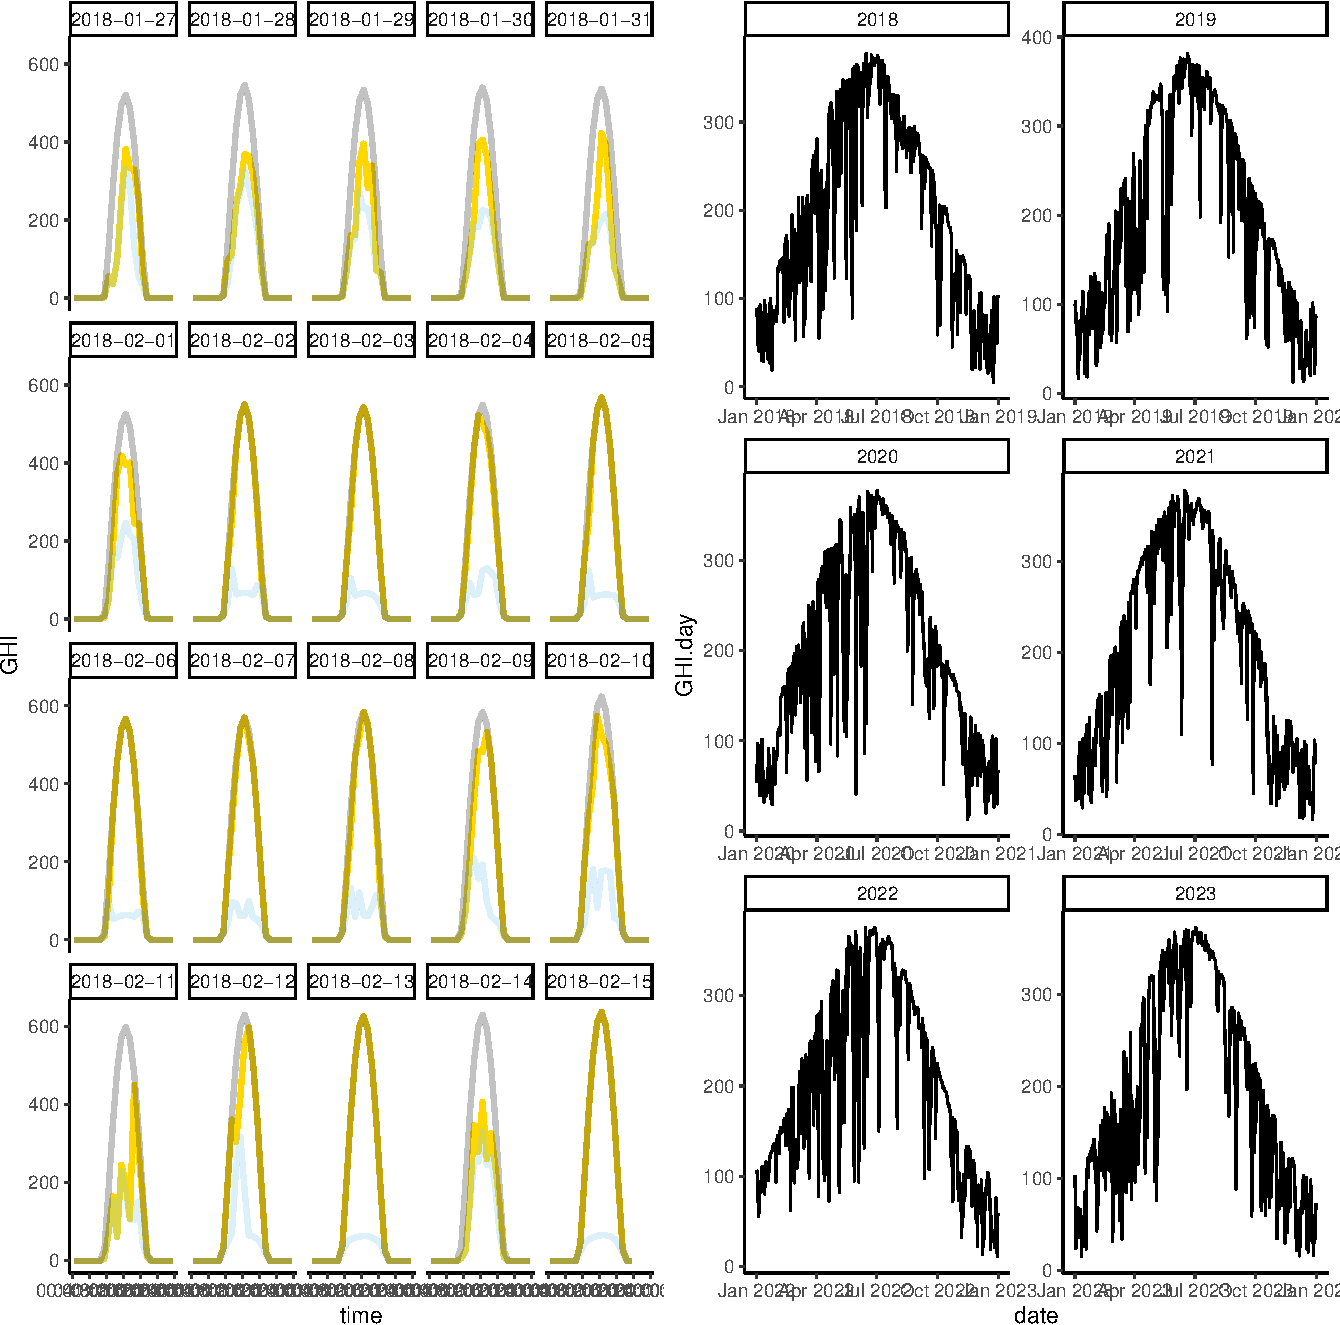
\includegraphics{Final_Metab_ModelOut_files/figure-pdf/unnamed-chunk-7-1.pdf}

\normalsize

\section{Run 1 diagnostics: Bayesian binned-Q
run}\label{run-1-diagnostics-bayesian-binned-q-run}

\subsection{First look at metabolism time series from the binned-Q
run}\label{first-look-at-metabolism-time-series-from-the-binned-q-run}

\begin{itemize}
\tightlist
\item
  Some +ER during high flows in winter
\item
  One period of weird +ER that may be due to biofouling
\item
  A few extreme estimates during the turbidity pulses
\item
  Overall, really nice, complete time series!
\end{itemize}

\small

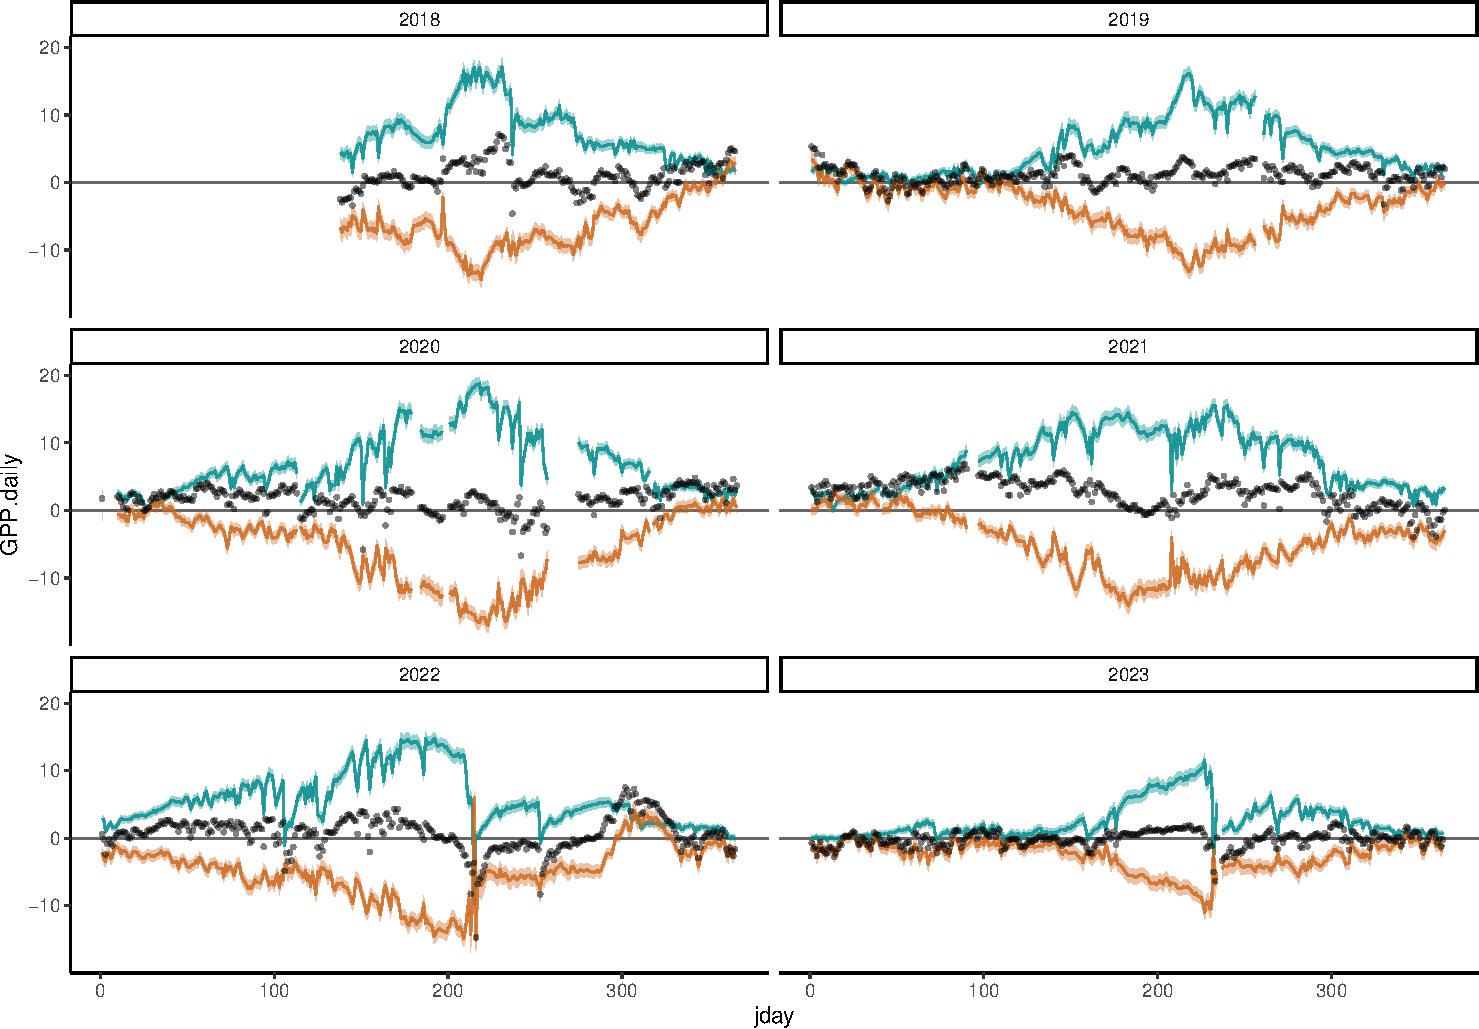
\includegraphics{Final_Metab_ModelOut_files/figure-pdf/unnamed-chunk-8-1.pdf}

\normalsize

\subsection{Model convergence diagnostics for the binned-Q
run}\label{model-convergence-diagnostics-for-the-binned-q-run}

\begin{itemize}
\tightlist
\item
  r\_hat values are all \textless{} 1.05
\item
  4 days had n\_eff \textless{} 200 but even these were 100 or more
\end{itemize}

\small

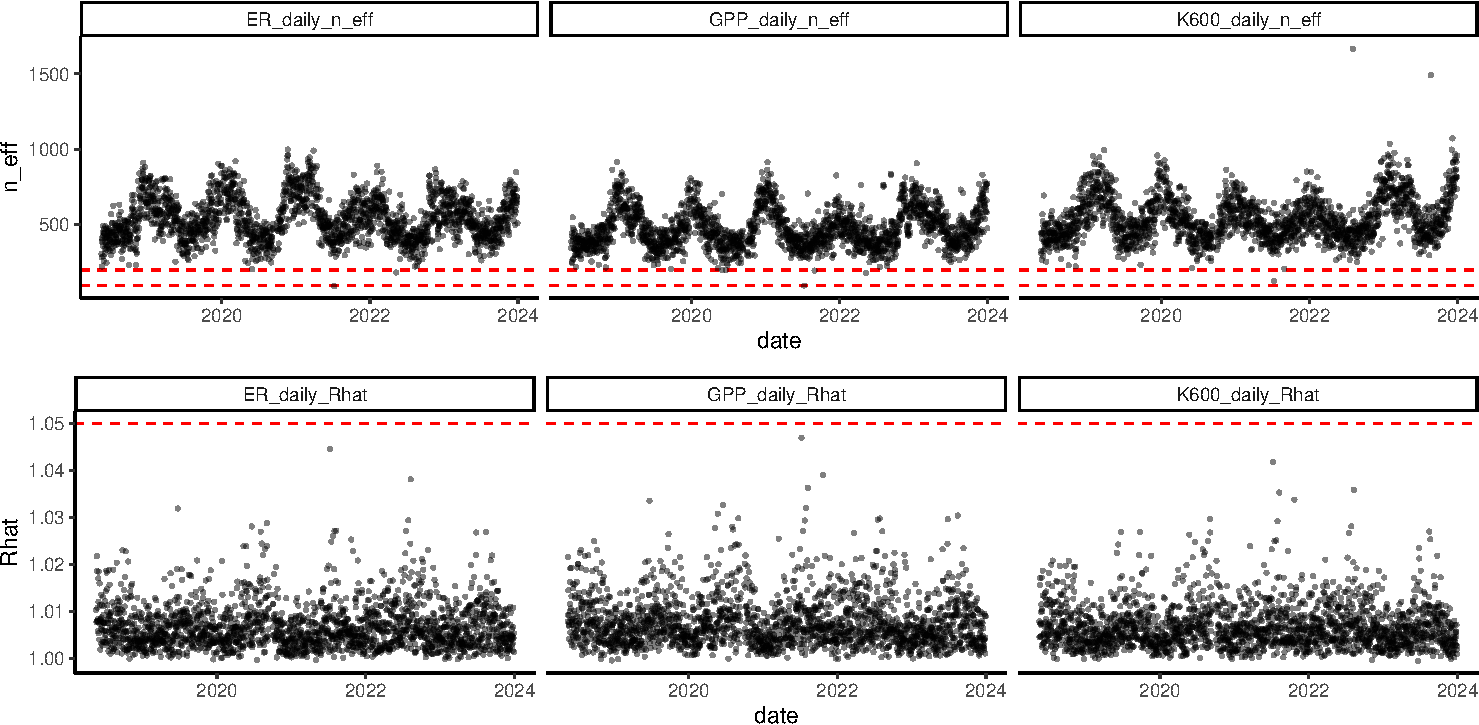
\includegraphics{Final_Metab_ModelOut_files/figure-pdf/unnamed-chunk-9-1.pdf}

\normalsize

\subsection{Model fits}\label{model-fits}

There is no standard cutoff, or even established metric for assessing
model fits for metabolism models. We used the normalized room mean
square error (NRMSE), because larger daily fluctuations in dissolved
O\(_2\) are more robust to model fit errors than days with small daily
fluctuations. We visually examined day with NRMSE \textgreater{} 0.15,
and looked at how well these poorer fits corresponded with day where
K600 fluctuated more than expected.

\subsubsection{NRMSE \textgreater{} 0.15}\label{nrmse-0.15}

\begin{itemize}
\tightlist
\item
  Plots show fits on all days with NRMSE \textgreater{} 0.15
\item
  Very few days with this level of poor fit (39 days)
\item
  Note the different y-axis for each panel
\end{itemize}

\small

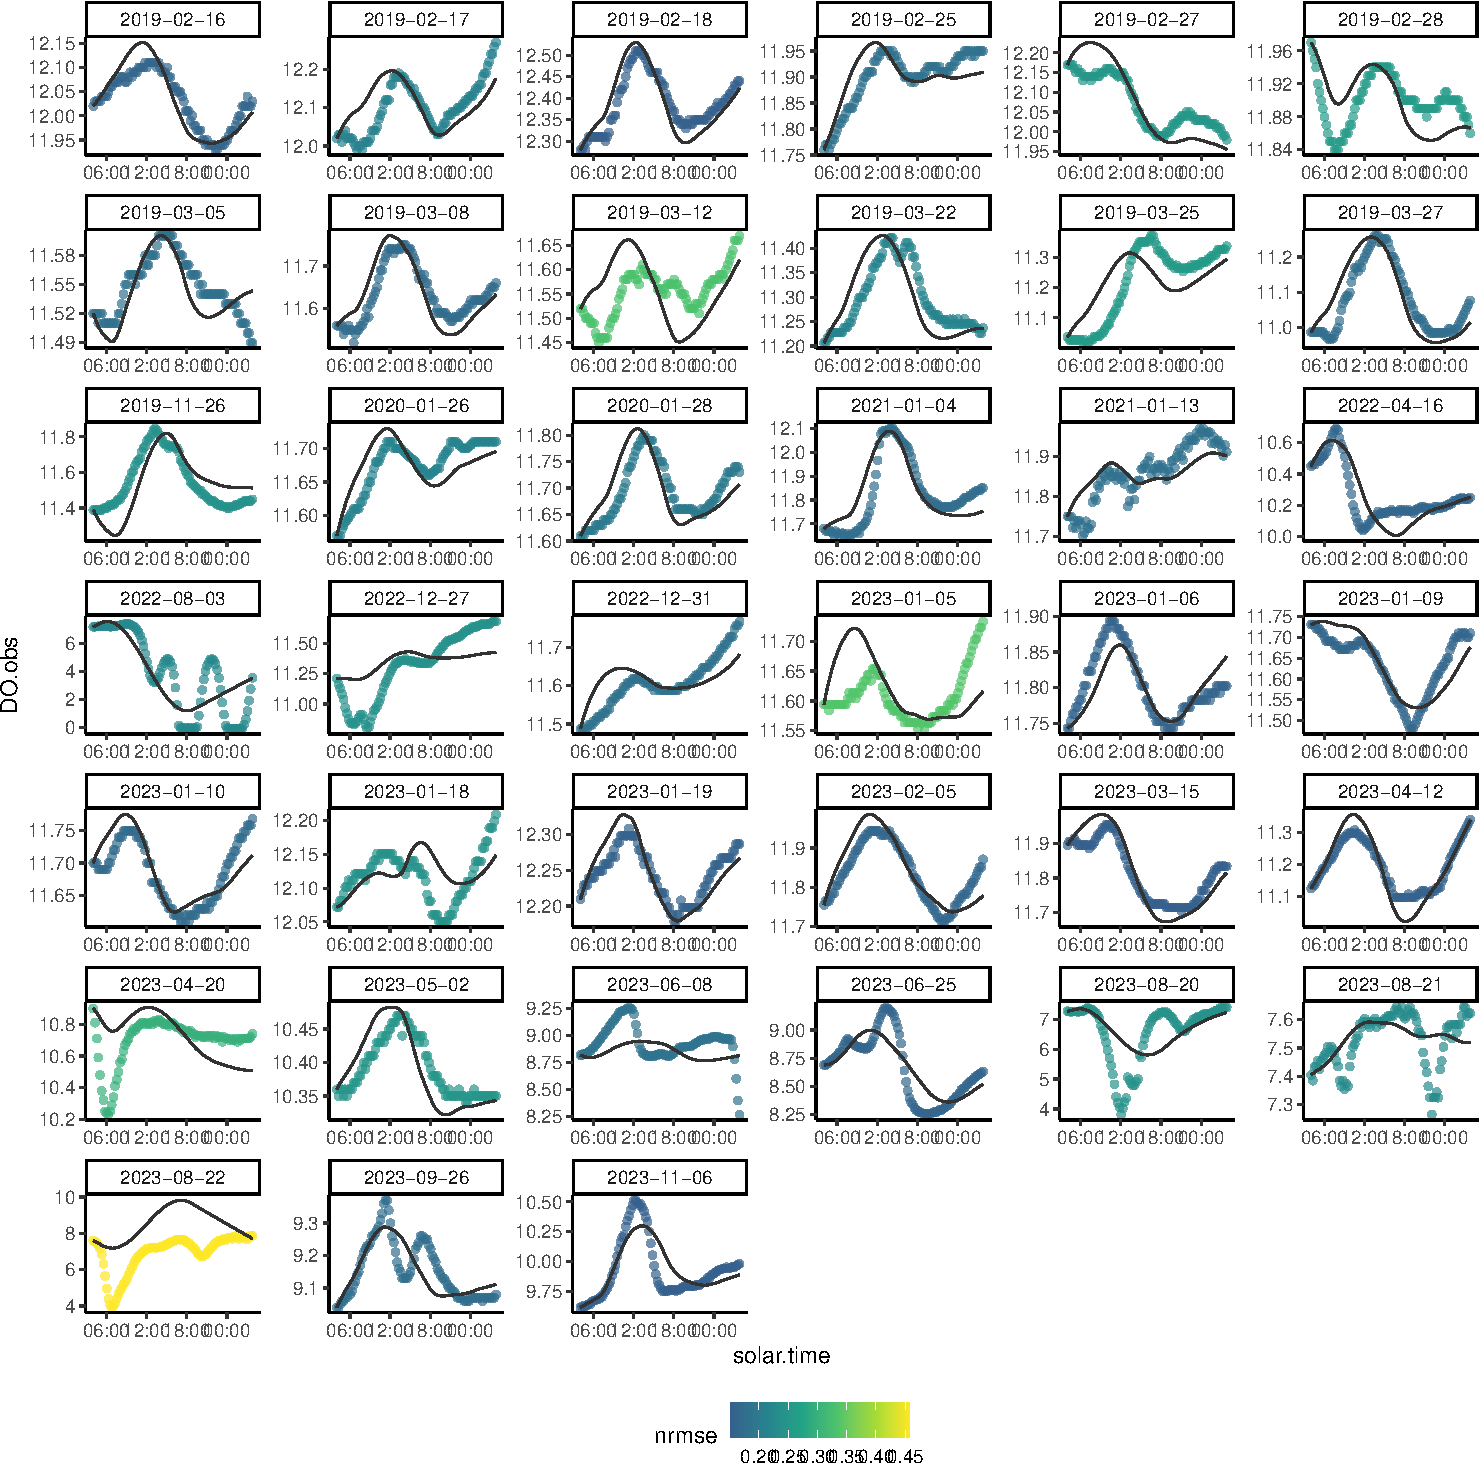
\includegraphics{Final_Metab_ModelOut_files/figure-pdf/unnamed-chunk-10-1.pdf}

\normalsize

\section{K600 values from the binned-Q
run}\label{k600-values-from-the-binned-q-run}

\subsection{K600 time series}\label{k600-time-series}

Red circles show days where NRMSE was \textgreater{} 0.15, while poor
fits explain some of the extreme points, the fits largely don't identify
a lot of funky K values, leading me to think that pooling by hand may be
our best option for this data set

\small


\includegraphics{Final_Metab_ModelOut_files/figure-pdf/unnamed-chunk-11-1.pdf}

\normalsize

\subsection{K600 by ER relationships}\label{k600-by-er-relationships}

Correlation between ER and K600 (\(r^2\) = 0.66); correlations are OK
due to flow. When flows are low, K600 is low and GPP is high, which
makes ER high. So it is biologically relevant, not due to overfitting of
K600 and ER.

\small

\begin{center}

\includegraphics{Final_Metab_ModelOut_files/figure-pdf/unnamed-chunk-12-1.pdf}
\end{center}

\normalsize

\subsection{K600 by year and by
discharge}\label{k600-by-year-and-by-discharge}

\begin{itemize}
\tightlist
\item
  Mean K600 = 11\(^{-d}\)
\item
  General trend of higher flow years having higher K\(_{600}\)
\item
  This is all good; data aligns with expectations here
\end{itemize}

\small

\begin{center}

\includegraphics{Final_Metab_ModelOut_files/figure-pdf/unnamed-chunk-13-1.pdf}
\end{center}

\normalsize

\subsection{K600 by discharge}\label{k600-by-discharge}

Relationship here is really clean; lowest K600 at lowest flows, with an
increase in gas exchange between 1000 to 2000 cfs, then it generally
level out across higher flows.

We have so many data points that we did not bother with eliminating the
few potential outliers that may have been attributed to poorer model
fits. Using fixed K600 from this relationship will fix this problem
entirely.

\small


\includegraphics{Final_Metab_ModelOut_files/figure-pdf/unnamed-chunk-14-1.pdf}

\normalsize

\subsection{Estimate K600 based on daily Q and rerun metabolism in
MLE}\label{estimate-k600-based-on-daily-q-and-rerun-metabolism-in-mle}

We used a loess relationship (shown in plot above) to estimate K600,
then export the K600 estimates and use them to model metabolism using
the MLE method. Metabolism estimates are done in ``SV-MetabCalcs.R''
script, in the second half of the script after the binned-Q run.

\small

\normalsize

\section{Compare MLE metabolism to
Bayes}\label{compare-mle-metabolism-to-bayes}

MLE and Bayes results are similar, but there is less day to day
variation in the MLE run, as expected, during peak GPP, the binned runs
often underestimate GPP and ER by a little bit. The CV for metabolism is
higher in the Bayes run than the hand-pooled K, but not hugely different
(CV for Bayes then MLE):

\begin{itemize}
\tightlist
\item
  K600: 0.17 vs.~0.13
\item
  ER: -0.95 vs.~-0.89
\item
  GPP: 0.75 vs.~0.78
\end{itemize}

\small

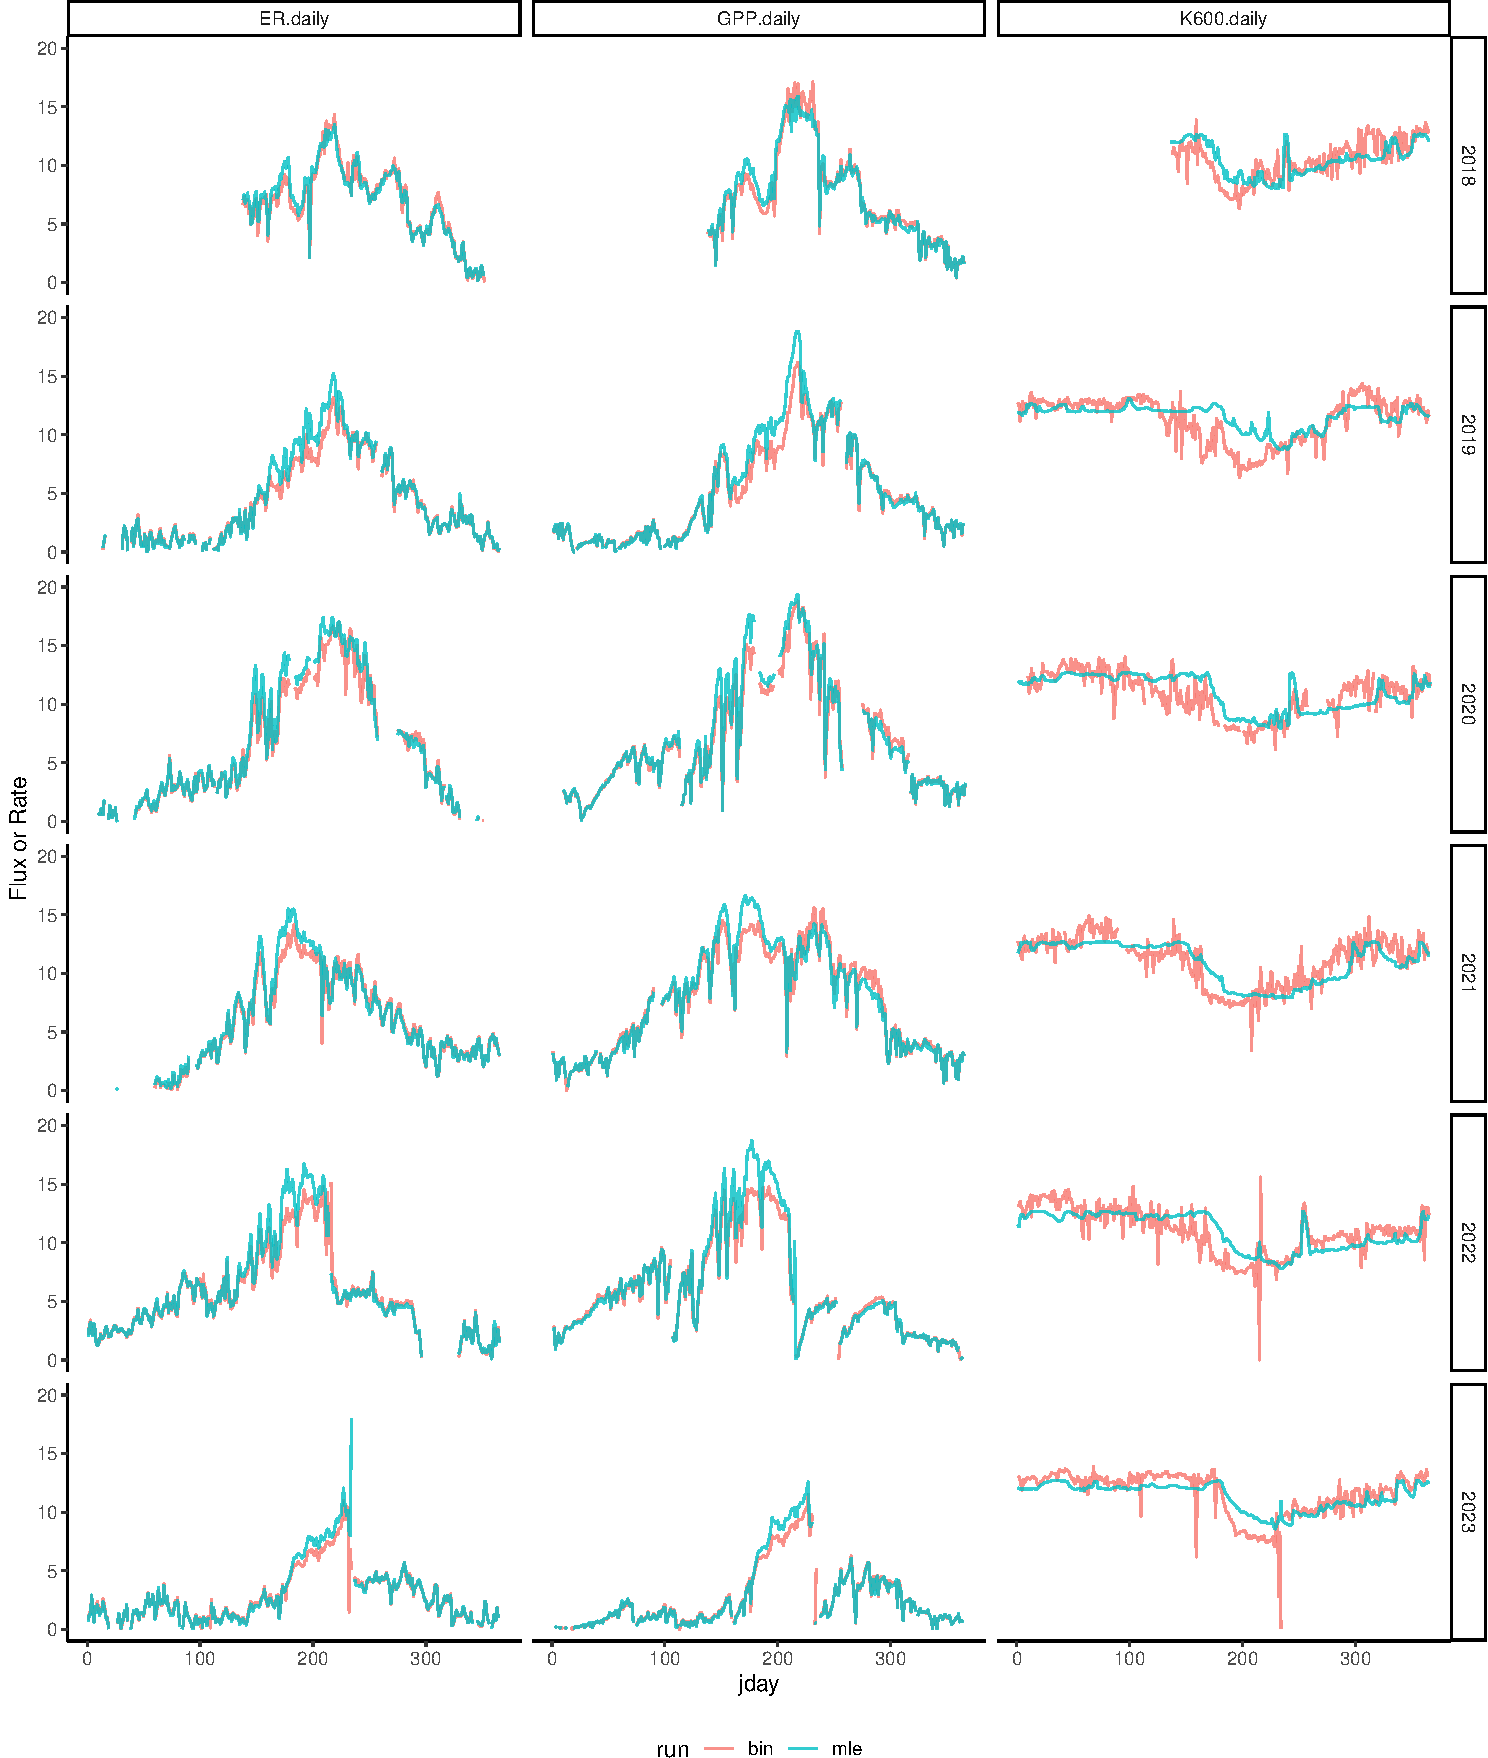
\includegraphics{Final_Metab_ModelOut_files/figure-pdf/unnamed-chunk-16-1.pdf}

\normalsize

\section{MLE metabolism model output}\label{mle-metabolism-model-output}

\subsection{MLE model fits}\label{mle-model-fits}

There is no standard cutoff, or even established metric for assessing
model fits for metabolism models. We used the normalized room mean
square error (NRMSE), because larger daily fluctuations in DO are more
robust to model fit errors than days with small daily fluctuations. In
looking at model fits with higher NRMSE scores, we find that most of
them are from days with very low DO exchange, and so even though there
may be some poor fits, they are overall still decent and give us the
same outcome: low metabolism. So, instead of using a cutoff in NRMSE, we
examined poor fit in the time series and only eliminated egregious fits
and fits that were poor and gave suspect (or blatantly unrealistic)
values of metabolism. Because we are not also estimating K600, we feel
pretty OK about model fits that are not perfect, as long as the DO on a
given day is governed by the assumptions of the metabolism equations.

\subsubsection{NRMSE \textgreater{} 0.1}\label{nrmse-0.1}

\begin{itemize}
\tightlist
\item
  Plots show fits on all days with NRMSE \textgreater{} 0.1
\item
  Very few days with this level of poor fit (111 days, most look great)
\item
  Note the different y-axis for each panel
\item
  NRMSE over-penalizes days with low DO change
\item
  Most days look pretty good, even here
\end{itemize}

\small

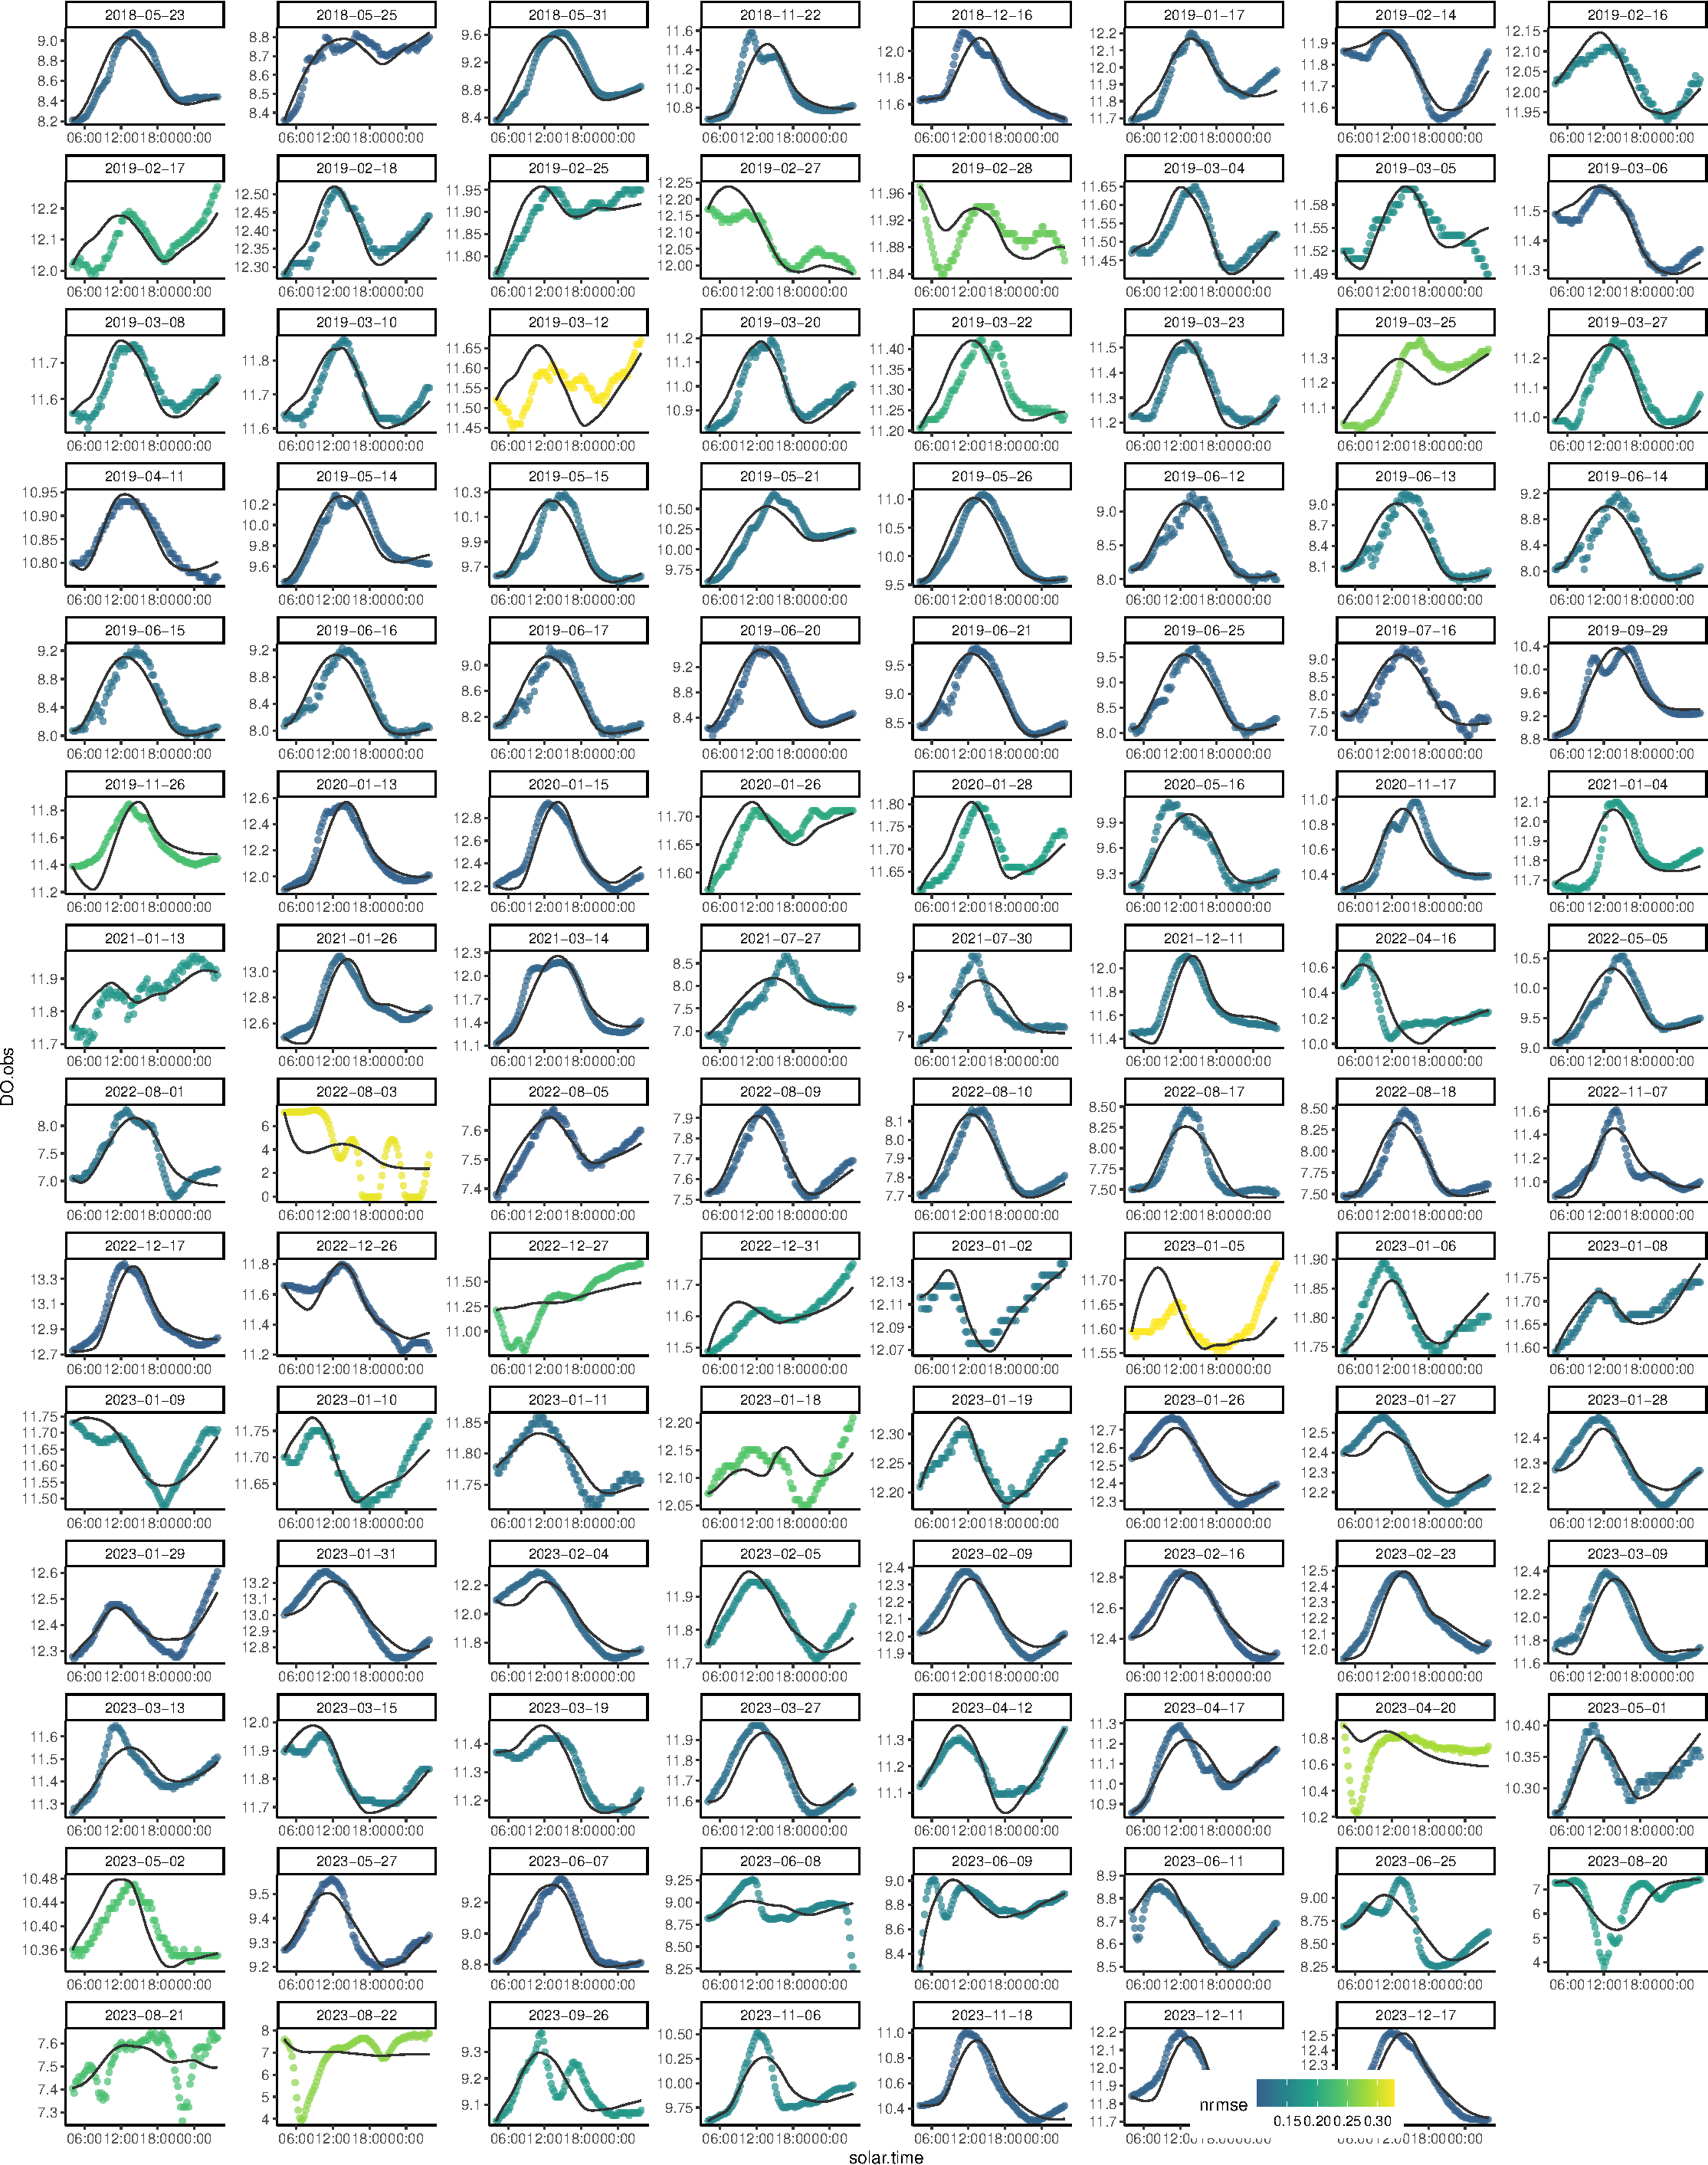
\includegraphics{Final_Metab_ModelOut_files/figure-pdf/unnamed-chunk-17-1.pdf}

\normalsize

\subsubsection{NRMSE at high DO
exchange}\label{nrmse-at-high-do-exchange}

Low is low, so I'm not worried about poor model fits when GPP is very
low. Only a few days are poor fits and correspond to funky values of GPP
including:

\begin{verbatim}
- 7/27/2021 and 7/30/2021 (big DO exchange; model missed the peaks)
- 8/3/2022 (Day of big turbidity pulse)
- 8/20/2023-8/22/2023 (2023 turbidity pulse)
\end{verbatim}

\small

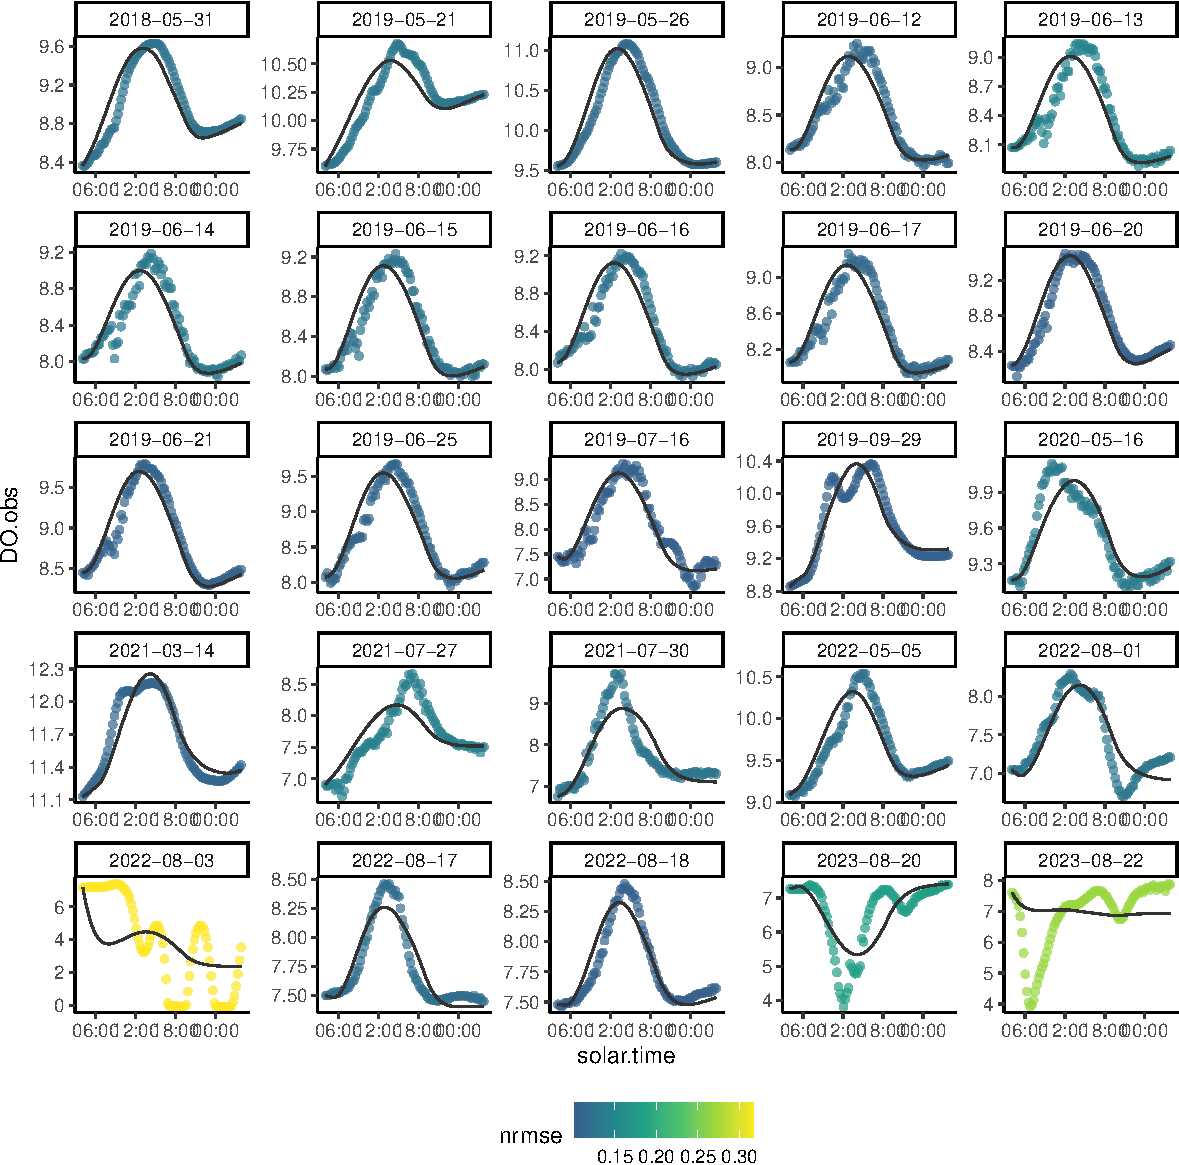
\includegraphics{Final_Metab_ModelOut_files/figure-pdf/unnamed-chunk-18-1.pdf}

\normalsize

\subsubsection{Time series of GPP with poor model fits in
purple}\label{time-series-of-gpp-with-poor-model-fits-in-purple}

I used this to identify where model fits affected the metabolism
estimates. Any fit with NMRSE \textgreater{} 0.1 is in purple, so most
of these fits are actually still pretty dang good, as shown in fit plots
above, but there are a few funky values the correspond to poor fits.

\small


\includegraphics{Final_Metab_ModelOut_files/figure-pdf/unnamed-chunk-19-1.pdf}

\normalsize

\subsubsection{Time series of ER with poor model fits in
purple}\label{time-series-of-er-with-poor-model-fits-in-purple}

\small


\includegraphics{Final_Metab_ModelOut_files/figure-pdf/unnamed-chunk-20-1.pdf}

\normalsize

\subsubsection{Positive ER and
super-saturation}\label{positive-er-and-super-saturation}

This shows where DO remains above 100\% saturation over a full 24 hour
period. This condition results in positive estimates of ER, but doesn't
affect GPP estimates. This only occurred in winter during higher
flows/colder temps, and during one fall period where some sort of
biofouling likely occurred that was possibly not identified by during
field calibrations--but we will likely never know.

In these occurrances, we flagged the ER data, but retain GPP values in
our data set.

\small


\includegraphics{Final_Metab_ModelOut_files/figure-pdf/unnamed-chunk-21-1.pdf}

\normalsize

\subsection{Dates to flag}\label{dates-to-flag}

While 111 (5\% of data set) days had model fits with an NRMSE
\textgreater{} 0.1, the vast majority of these days had poor NRMSE
scores due to very small daily DO fluctuation, indicating low
metabolism. In order to not eliminate days where metabolism was very low
but estimates were very likely good, we examined poor model fits in the
time series, and only eliminated days where model fits were poor and
caused values of GPP and ER that were unlikely given the surrounding
data points, or that produced biologically impossible estimates of GPP
and/or ER. This resulted in just 7 days being flagged for poor model
fits.

\begin{itemize}
\tightlist
\item
  2021-07-27
\item
  2021-07-30
\item
  2022-04-16
\item
  2022-08-03
\item
  2023-08-20
\item
  2023-08-21
\item
  2023-08-22
\end{itemize}

The 2021 dates appear to have had a cold front move in, likely
depressing GPP as predicted, but model fits were sufficiently poor to
not trust estimates, despite the downward shift in GPP those days being
likely.

In 2022, the April date had a relatively small DO exchange, and model
fit was not egregious, but the daily pattern was irregular, suggesting
mid-day shifts in process the produced a negative GPP estimate. August
of 2022 was the day of the huge turbidity pulse, with highly irregular
within day DO consumption.

August 2023 had a huge turbidity pulse due to more rain on the McKinney
Fire scar, making for weird DO that the model didn't like.

Fits for these 7 days plotted below:

\small

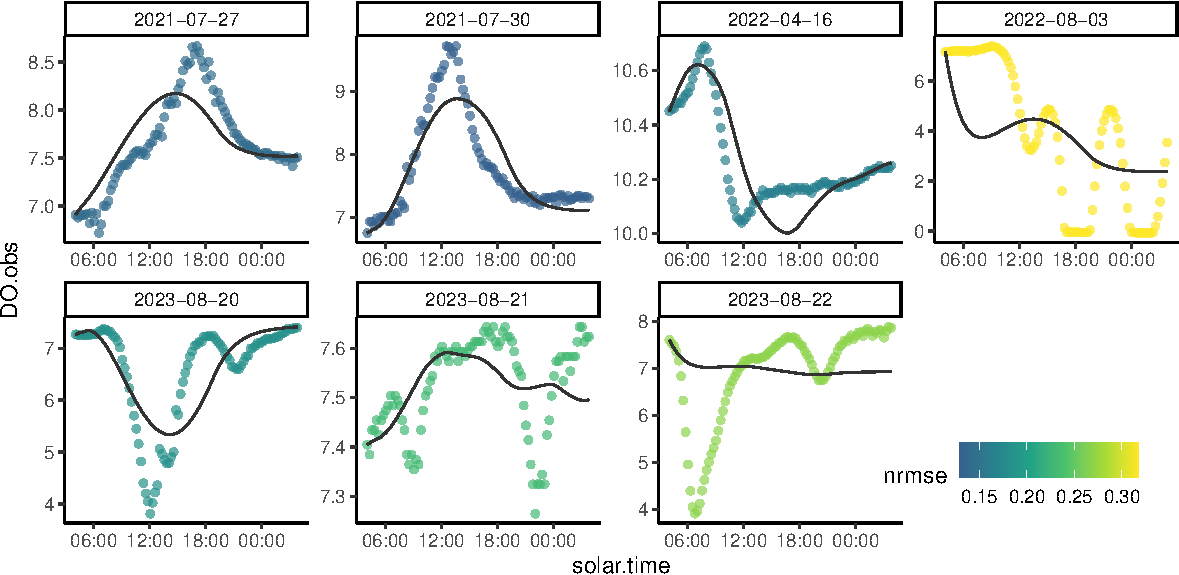
\includegraphics{Final_Metab_ModelOut_files/figure-pdf/unnamed-chunk-22-1.pdf}

\normalsize

\subsection{Flag QA'd data (bad model fits and unrealistic
estimates)}\label{flag-qad-data-bad-model-fits-and-unrealistic-estimates}

\begin{itemize}
\tightlist
\item
  Flag dates with poor model fits from visual examination above (7 days)
\item
  Flag ER with min daily saturation \textgreater{} 100\% (this applies
  to ER only; 155 days)
\item
  Check how many values are above/below 0 after filtering these points
  above--

  \begin{itemize}
  \tightlist
  \item
    ER: 55 days \textgreater{} 0; 44 where the lower limit is
    \textgreater{} 0
  \item
    GPP: 24 days \textless{} 0; 14 where the upper limit is \textless{}
    0
  \end{itemize}

  I'm not going to worry about flagging additional days for unrealistic
  values b/c there were no estimates of GPP that were beyond -1, and
  only 4 days of ER were beyond 1 and those were still quite low (less
  than \textasciitilde2)--these are well within the error expected on
  other days and will not change the conclusions of the analysis.
\end{itemize}

\small

\normalsize

\section{Final time series}\label{final-time-series}

\begin{itemize}
\tightlist
\item
  Grey points passed the QA
\item
  Orange points exclude ER (and NEP) only
\item
  Red points exclude ER and GPP
\end{itemize}

\small

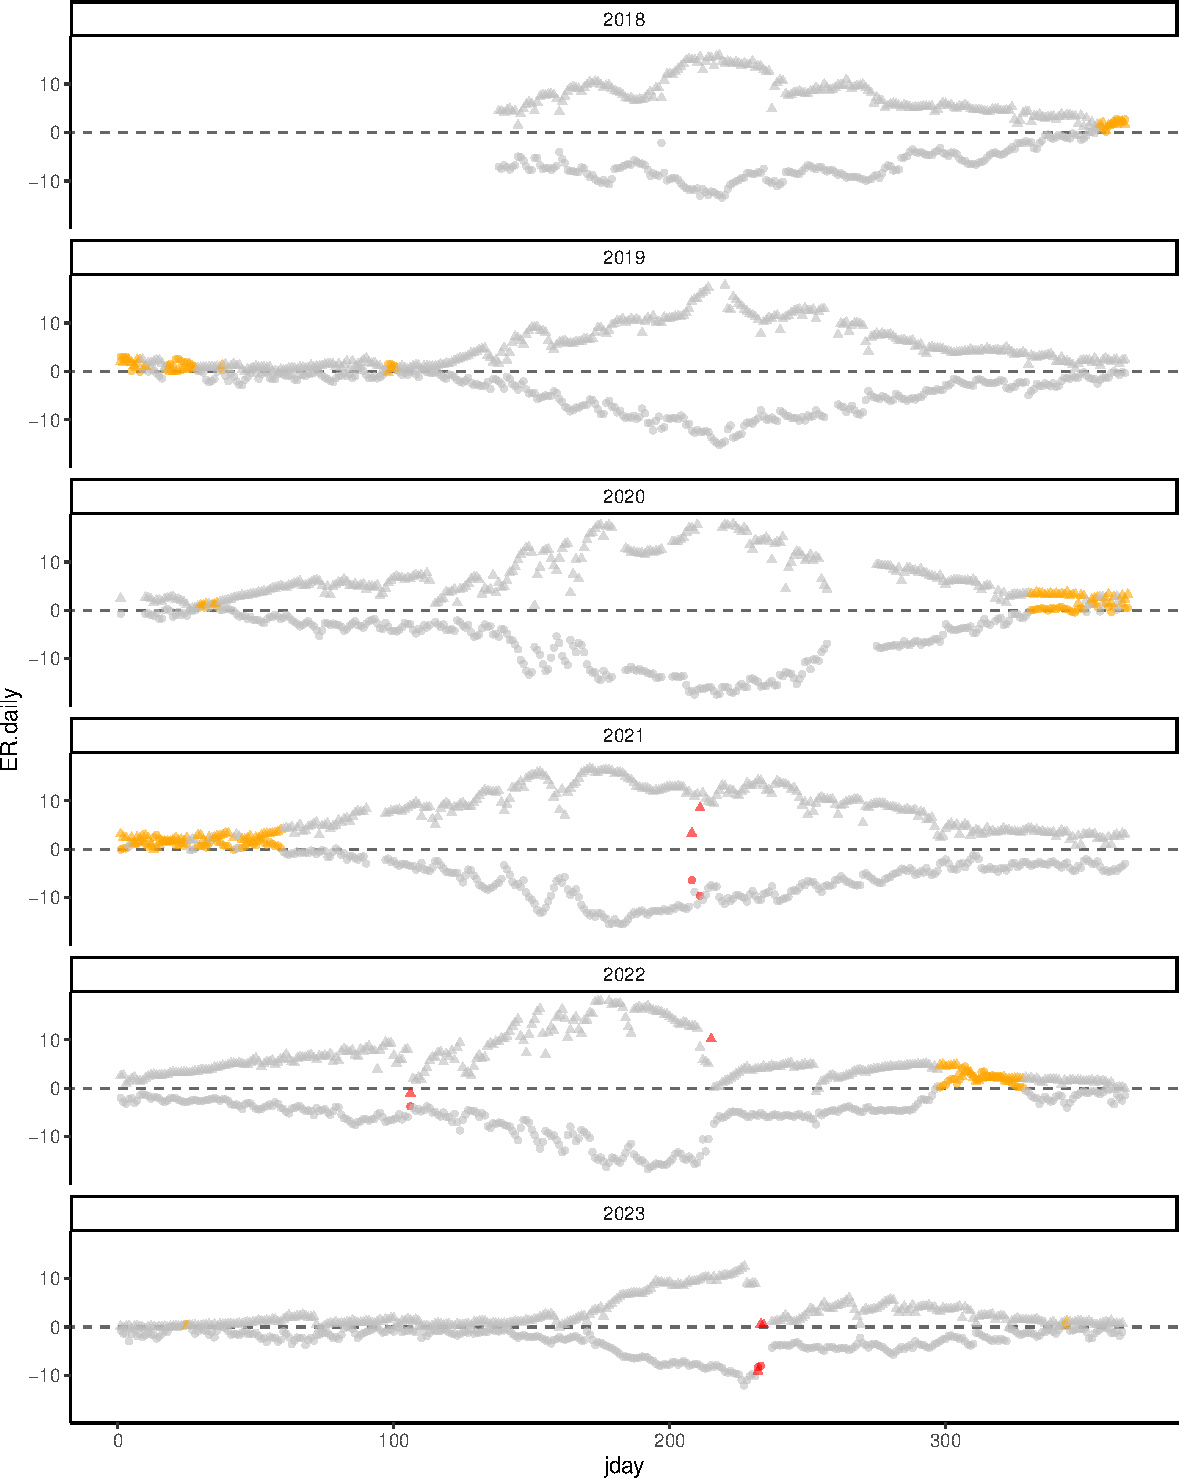
\includegraphics{Final_Metab_ModelOut_files/figure-pdf/unnamed-chunk-24-1.pdf}

\normalsize

\subsection{Build the data frame}\label{build-the-data-frame}

\begin{itemize}
\tightlist
\item
  Calc. NEP
\item
  Scale ER, GPP, and NEP to depth {[}z \textless- exp(-1.47 + 0.45 *
  log(40)){]}
\item
  Bin light
\item
  Only save columns used in McK-Fire analysis
\item
  Will need to filter out QA days in figures and analysis scripts; QA
  codes are included in the final data frame here.
\end{itemize}

\small

\begin{Shaded}
\begin{Highlighting}[]
\NormalTok{sv.wq.relevant }\OtherTok{\textless{}{-}}\NormalTok{ sv.wq }\SpecialCharTok{\%\textgreater{}\%}\NormalTok{ dplyr}\SpecialCharTok{::} \FunctionTok{select}\NormalTok{(date, turb\_min, turb\_median, turb\_max)}

\NormalTok{met.mle.final }\OtherTok{\textless{}{-}}\NormalTok{ met.mle.QA}\SpecialCharTok{\%\textgreater{}\%}
  \FunctionTok{mutate}\NormalTok{(}\AttributeTok{SV.cms =}\NormalTok{ SV.cfs }\SpecialCharTok{*} \FloatTok{0.0283168}\NormalTok{)}\SpecialCharTok{\%\textgreater{}\%}
  \FunctionTok{mutate}\NormalTok{(}\AttributeTok{z =} \FunctionTok{exp}\NormalTok{(}\SpecialCharTok{{-}}\FloatTok{1.47} \SpecialCharTok{+} \FloatTok{0.45} \SpecialCharTok{*} \FunctionTok{log}\NormalTok{(SV.cms)))}\SpecialCharTok{\%\textgreater{}\%}
  \FunctionTok{mutate}\NormalTok{(}\AttributeTok{GPP =}\NormalTok{ GPP.daily}\SpecialCharTok{*}\NormalTok{z,}
         \AttributeTok{GPP.upper =}\NormalTok{ GPP.daily.upper}\SpecialCharTok{*}\NormalTok{z,}
         \AttributeTok{GPP.lower =}\NormalTok{ GPP.daily.lower}\SpecialCharTok{*}\NormalTok{z,}
         \AttributeTok{ER =}\NormalTok{ ER.daily}\SpecialCharTok{*}\NormalTok{z,}
         \AttributeTok{ER.upper =}\NormalTok{ ER.daily.upper}\SpecialCharTok{*}\NormalTok{z,}
         \AttributeTok{ER.lower =}\NormalTok{ ER.daily.lower}\SpecialCharTok{*}\NormalTok{z)}\SpecialCharTok{\%\textgreater{}\%}
  \FunctionTok{mutate}\NormalTok{(}\AttributeTok{NEP =}\NormalTok{ GPP }\SpecialCharTok{+}\NormalTok{ ER)}\SpecialCharTok{\%\textgreater{}\%}
\NormalTok{ dplyr}\SpecialCharTok{::}\FunctionTok{select}\NormalTok{(GPP, GPP.upper, GPP.lower, ER, ER.upper, ER.lower, NEP, K600.daily, }
\NormalTok{         SV.cfs, IG.cfs, SV.cms, z, }
\NormalTok{         date, year, water.year, jday, mon,}
\NormalTok{         min.DO, QA.code)}\SpecialCharTok{\%\textgreater{}\%}
  \FunctionTok{left\_join}\NormalTok{(PAR.Day, }\AttributeTok{by =} \StringTok{"date"}\NormalTok{)}\SpecialCharTok{\%\textgreater{}\%}
  \FunctionTok{left\_join}\NormalTok{(sv.wq.relevant, }\AttributeTok{by =} \StringTok{"date"}\NormalTok{)}\SpecialCharTok{\%\textgreater{}\%}
\NormalTok{  dplyr}\SpecialCharTok{::}\FunctionTok{select}\NormalTok{(}
\NormalTok{    date, year, water.year, mon, jday,}
\NormalTok{    GPP, GPP.lower, GPP.upper, ER, ER.lower, ER.upper, NEP, K600.daily,}
\NormalTok{  SV.cfs, SV.cms, z, min.DO, GHI.day, turb\_min, turb\_median, turb\_max, QA.code)}\SpecialCharTok{\%\textgreater{}\%}
 \FunctionTok{mutate}\NormalTok{(}\FunctionTok{across}\NormalTok{(}\FunctionTok{c}\NormalTok{(GPP, GPP.lower, GPP.upper,}
\NormalTok{        ER, ER.lower, ER.upper, NEP, K600.daily, SV.cms),}
      \SpecialCharTok{\textasciitilde{}} \FunctionTok{round}\NormalTok{(.x, }\DecValTok{1}\NormalTok{)))}\SpecialCharTok{\%\textgreater{}\%}
   \FunctionTok{mutate}\NormalTok{(}\FunctionTok{across}\NormalTok{(}\FunctionTok{c}\NormalTok{(z, turb\_min, turb\_median, turb\_max), }\SpecialCharTok{\textasciitilde{}} \FunctionTok{round}\NormalTok{(.x, }\DecValTok{2}\NormalTok{)))}\SpecialCharTok{\%\textgreater{}\%}
  \FunctionTok{mutate}\NormalTok{(}\FunctionTok{across}\NormalTok{(}\FunctionTok{c}\NormalTok{(GHI.day,), }\SpecialCharTok{\textasciitilde{}} \FunctionTok{round}\NormalTok{(.x, }\DecValTok{0}\NormalTok{)))}\SpecialCharTok{\%\textgreater{}\%}
  \FunctionTok{mutate}\NormalTok{(}\FunctionTok{across}\NormalTok{(}\FunctionTok{c}\NormalTok{(min.DO), }\SpecialCharTok{\textasciitilde{}} \FunctionTok{round}\NormalTok{(.x, }\DecValTok{3}\NormalTok{)))}
\end{Highlighting}
\end{Shaded}

\normalsize

\subsection{Write the final metab data
frame}\label{write-the-final-metab-data-frame}

\small

\begin{Shaded}
\begin{Highlighting}[]
\FunctionTok{write.csv}\NormalTok{(met.mle.final, }\StringTok{"Data/met\_mle\_final.csv"}\NormalTok{)}
\end{Highlighting}
\end{Shaded}

\normalsize

\section{Short term high freq data}\label{short-term-high-freq-data}

This is the data for figure 1; during the sediment pulse. 6 days of high
frequency data to show what happened during the big sediment pulse.

\subsection{Load data and combine to produce the figure 1 data
frame}\label{load-data-and-combine-to-produce-the-figure-1-data-frame}

\small

\begin{Shaded}
\begin{Highlighting}[]
\NormalTok{svq.sub }\OtherTok{\textless{}{-}} \FunctionTok{readNWISuv}\NormalTok{(}
  \AttributeTok{siteNumbers =} \StringTok{"11520500"}\NormalTok{,}
  \AttributeTok{parameterCd =} \StringTok{"00060"}\NormalTok{,    }
  \AttributeTok{startDate =} \StringTok{"2022{-}07{-}31"}\NormalTok{,}
  \AttributeTok{endDate =} \StringTok{"2022{-}08{-}05"}\NormalTok{) }\SpecialCharTok{\%\textgreater{}\%}
\NormalTok{  dplyr}\SpecialCharTok{::}\FunctionTok{select}\NormalTok{(dateTime, X\_00060\_00000) }\SpecialCharTok{\%\textgreater{}\%} 
  \FunctionTok{rename}\NormalTok{(}\AttributeTok{datetime =}\NormalTok{ dateTime, }\AttributeTok{SV.cfs =}\NormalTok{ X\_00060\_00000) }\SpecialCharTok{\%\textgreater{}\%}
  \FunctionTok{mutate}\NormalTok{(}\AttributeTok{datetime =} \FunctionTok{as.POSIXct}\NormalTok{(datetime, }\AttributeTok{tz =} \StringTok{\textquotesingle{}Etc/GMT+7\textquotesingle{}}\NormalTok{))}

\NormalTok{sv.sonde }\OtherTok{\textless{}{-}} \FunctionTok{read\_csv}\NormalTok{(}\StringTok{"Data/SV\_2018{-}2024\_AllParams.csv"}\NormalTok{, }\AttributeTok{skip =} \DecValTok{16}\NormalTok{, }\AttributeTok{col\_names =} \FunctionTok{c}\NormalTok{(}\StringTok{"dtime"}\NormalTok{, }\StringTok{"temp.water"}\NormalTok{, }\StringTok{"sc"}\NormalTok{, }\StringTok{"domg"}\NormalTok{, }\StringTok{"ph"}\NormalTok{, }\StringTok{"turb"}\NormalTok{))}\SpecialCharTok{\%\textgreater{}\%}
            \FunctionTok{separate}\NormalTok{(dtime, }\AttributeTok{into =} \FunctionTok{c}\NormalTok{(}\StringTok{"date"}\NormalTok{, }\StringTok{"time"}\NormalTok{), }\AttributeTok{sep =} \StringTok{" "}\NormalTok{, }\AttributeTok{remove =}\NormalTok{ F)}\SpecialCharTok{\%\textgreater{}\%}
  \FunctionTok{mutate}\NormalTok{(}\AttributeTok{datetime =} \FunctionTok{force\_tz}\NormalTok{(dtime, }\AttributeTok{tz=}\StringTok{\textquotesingle{}Etc/GMT+7\textquotesingle{}}\NormalTok{))}\SpecialCharTok{\%\textgreater{}\%}
  \FunctionTok{mutate}\NormalTok{(}\AttributeTok{date =} \FunctionTok{as.Date}\NormalTok{(date))}\SpecialCharTok{\%\textgreater{}\%}
  \FunctionTok{filter}\NormalTok{(date }\SpecialCharTok{\textgreater{}=} \FunctionTok{as.Date}\NormalTok{(}\StringTok{"2022{-}07{-}30"}\NormalTok{) }\SpecialCharTok{\&}\NormalTok{ date }\SpecialCharTok{\textless{}=} \FunctionTok{as.Date}\NormalTok{(}\StringTok{"2022{-}08{-}05"}\NormalTok{))}

\NormalTok{sv.light }\OtherTok{\textless{}{-}}\NormalTok{ PAR }\SpecialCharTok{\%\textgreater{}\%}
\NormalTok{  dplyr}\SpecialCharTok{::}\FunctionTok{select}\NormalTok{(time, date, GHI) }\SpecialCharTok{\%\textgreater{}\%}
  \FunctionTok{filter}\NormalTok{(date }\SpecialCharTok{\textgreater{}=} \FunctionTok{as.Date}\NormalTok{(}\StringTok{"2022{-}07{-}30"}\NormalTok{) }\SpecialCharTok{\&}\NormalTok{ date }\SpecialCharTok{\textless{}=} \FunctionTok{as.Date}\NormalTok{(}\StringTok{"2022{-}08{-}05"}\NormalTok{)) }\SpecialCharTok{\%\textgreater{}\%}
  \FunctionTok{mutate}\NormalTok{(}\AttributeTok{datetime =} \FunctionTok{ymd\_hms}\NormalTok{(}\FunctionTok{paste}\NormalTok{(date, time)),}
    \AttributeTok{datetime =} \FunctionTok{force\_tz}\NormalTok{(datetime, }\AttributeTok{tzone =} \StringTok{"Etc/GMT+7"}\NormalTok{))}\SpecialCharTok{\%\textgreater{}\%}
\NormalTok{  dplyr}\SpecialCharTok{::}\FunctionTok{select}\NormalTok{(}\SpecialCharTok{{-}}\NormalTok{time)}
  
\NormalTok{sub.day }\OtherTok{\textless{}{-}}\NormalTok{ svq.sub }\SpecialCharTok{\%\textgreater{}\%} 
  \FunctionTok{left\_join}\NormalTok{(sv.sonde, }\AttributeTok{by =} \FunctionTok{c}\NormalTok{(}\StringTok{"datetime"}\NormalTok{))}\SpecialCharTok{\%\textgreater{}\%}
  \FunctionTok{left\_join}\NormalTok{(sv.light, }\AttributeTok{by =} \FunctionTok{c}\NormalTok{(}\StringTok{"datetime"}\NormalTok{, }\StringTok{"date"}\NormalTok{))}\SpecialCharTok{\%\textgreater{}\%}
  \FunctionTok{mutate}\NormalTok{(}\AttributeTok{GHI\_interp =} \FunctionTok{na.approx}\NormalTok{(GHI, }\AttributeTok{x =}\NormalTok{ datetime, }\AttributeTok{na.rm =} \ConstantTok{FALSE}\NormalTok{, }\AttributeTok{rule =} \DecValTok{10}\NormalTok{))}\SpecialCharTok{\%\textgreater{}\%}
\NormalTok{  dplyr}\SpecialCharTok{::}\FunctionTok{select}\NormalTok{(datetime, GHI, GHI\_interp, SV.cfs, domg, turb)}\SpecialCharTok{\%\textgreater{}\%}
   \FunctionTok{mutate}\NormalTok{(}\FunctionTok{across}\NormalTok{(}\FunctionTok{c}\NormalTok{(GHI, GHI\_interp), }\SpecialCharTok{\textasciitilde{}} \FunctionTok{round}\NormalTok{(.x, }\DecValTok{0}\NormalTok{)))}\SpecialCharTok{\%\textgreater{}\%}
  \FunctionTok{mutate}\NormalTok{(}\FunctionTok{across}\NormalTok{(}\FunctionTok{c}\NormalTok{(turb), }\SpecialCharTok{\textasciitilde{}} \FunctionTok{round}\NormalTok{(.x, }\DecValTok{2}\NormalTok{)))}

\CommentTok{\#write.csv(sub.day, "Data/sub{-}daily{-}FIRE.csv")}
\end{Highlighting}
\end{Shaded}

\normalsize

\section{Reach length estimates}\label{reach-length-estimates}

Estimating reach lengths based on the dissolved oxygen turnover
distance. We calculated the reach lenght at 1860 cfs which is about the
50\% exceedance flow, using the K600 from the Loess at that flow, depth
as estimated from the depth model, and velocity from Jenny Curtis's USGS
report.

\begin{itemize}
\tightlist
\item
  Curtis data collected June 11-13; 1860 cfs on June 12, 2018
\item
  K600 at 1860, based on Loess of Q/K600 from bayes run: 12.7
\item
  1870 cfs is 50\% exceedance prob flow for SV
\end{itemize}

Estimates of reach length are 8.2 km for the 80\% turnover distance and
15.4 for the 95\% turnover distance, so I used 10km as my reach length.

\small

\begin{Shaded}
\begin{Highlighting}[]
\NormalTok{geom }\OtherTok{\textless{}{-}} \FunctionTok{read.csv}\NormalTok{(}\StringTok{"Data/Depth/Summary\_Table\_Geomorphology\_and\_Land\_Surface\_Parameters\_Klamath\_River\_California\_2018.csv"}\NormalTok{)}

\NormalTok{geom }\SpecialCharTok{\%\textgreater{}\%} \FunctionTok{filter}\NormalTok{(RKM\_Reach\_ID }\SpecialCharTok{\%in\%} \FunctionTok{c}\NormalTok{(}\DecValTok{93}\SpecialCharTok{:}\DecValTok{102}\NormalTok{))}\SpecialCharTok{\%\textgreater{}\%}
  \FunctionTok{summarize}\NormalTok{(}\AttributeTok{w =} \FunctionTok{mean}\NormalTok{(Channel\_Width\_m))}\SpecialCharTok{\%\textgreater{}\%}
  \FunctionTok{mutate}\NormalTok{(}\AttributeTok{cms =} \DecValTok{1860}\SpecialCharTok{/}\FloatTok{35.3146}\NormalTok{,}
         \AttributeTok{z =} \FunctionTok{exp}\NormalTok{(}\SpecialCharTok{{-}}\FloatTok{1.47} \SpecialCharTok{+} \FloatTok{0.45} \SpecialCharTok{*} \FunctionTok{log}\NormalTok{(cms)),}
         \AttributeTok{v =}\NormalTok{ cms}\SpecialCharTok{/}\NormalTok{(w}\SpecialCharTok{*}\NormalTok{z),}
         \AttributeTok{fp80 =}\NormalTok{ (}\FloatTok{1.6}\SpecialCharTok{*}\NormalTok{v}\SpecialCharTok{*}\DecValTok{86400}\NormalTok{)}\SpecialCharTok{/}\FloatTok{12.7}\NormalTok{,}
         \AttributeTok{fp95 =}\NormalTok{ (}\DecValTok{3}\SpecialCharTok{*}\NormalTok{v}\SpecialCharTok{*}\DecValTok{86400}\NormalTok{)}\SpecialCharTok{/}\FloatTok{12.7}\NormalTok{)}
\end{Highlighting}
\end{Shaded}

\begin{verbatim}
       w      cms        z         v     fp80     fp95
1 50.863 52.66943 1.368638 0.7566032 8235.656 15441.85
\end{verbatim}

\normalsize




\end{document}
